\section{Scale sensitivity}\label{sec:sensitivity}

No construction evaluates its half-width at the truth. Each evaluates it at a
bound. \textbf{What separates constructions is therefore not how well they
estimate the scale---they can be given the same estimate---but how hard the
interval reacts to being wrong about it.}

\begin{definition}
For a half-width $R$ depending on a scale $\theta$, the \emph{scale elasticity}
is $e(\theta)=\partial\log R/\partial\log\theta$.
\end{definition}

\paragraph{What is held fixed.} The derivative is taken in the scale at which
the half-width is \emph{evaluated}, with the data---and hence the empirical
radius $q=\operatorname{ord}_m|Y_c|$ of \eqref{eq:band}---held fixed. It is not
the derivative of the oracle width: at the truth every construction here has
half-width proportional to $\sqrt A$ and so oracle elasticity $1/2$. The
distinction is the substance of this section. Constructions can be given the same
information about the scale and still differ in how an error in the plugged-in
bound propagates into the number they report, and it is that propagation, not the
quality of the estimate, that decides which is narrower.

With latent scale $A$ and design variance $L$, so $\rho^2=L/(A+L)$:

\begin{center}
\begin{tabular}{lll}
\toprule
construction & half-width & elasticity in $A$\\
\midrule
deconvolution band & $q\sqrt{A/(A+L)}$ & $L/\{2(A+L)\}=\rho^2/2$\\
any band $\propto\sqrt A$ & $z\sqrt A$ & $1/2$\\
uncorrected anchor & $q$ & $0$\\
\bottomrule
\end{tabular}
\end{center}

The deconvolution band's elasticity is \textbf{damped by the design share}. This
is not a property of conformal prediction: it follows from dividing by
$\sqrt{A+L}$ and multiplying by $\sqrt A$, and any construction of that form
inherits it.

Figure~\ref{fig:elasticity} shows both halves of the claim: the relative cost of
a loose bound on the left, and on the right the elasticity measured in eight
simulation cells against the predicted $\rho^2/2$. The measurement sits below
the prediction in every cell, averaging $0.86$ of it---the damping is real and is
slightly stronger than the first-order calculation says, which is the safe
direction for a claim of the form ``this construction reacts less''.

\begin{figure}[t]
\centering
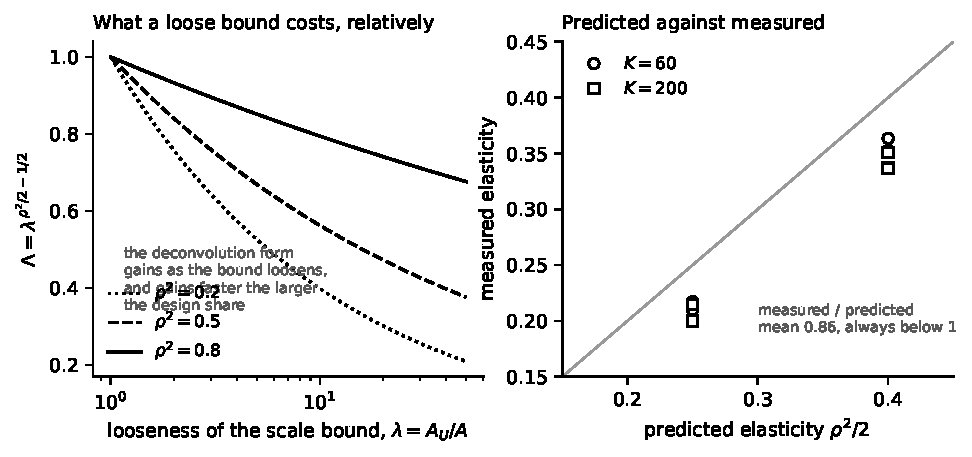
\includegraphics[width=\textwidth]{figures/fig1_elasticity}
\caption{\textbf{Left:} the exchange identity of
Proposition~\ref{prop:exchange}. Evaluated at a bound loose by $\lambda$, the
deconvolution band's half-width moves by $\lambda^{\rho^2/2}$ where a band
proportional to $\sqrt{A}$ moves by $\lambda^{1/2}$; the curves are their exact
ratio, with no fitted constant. \textbf{Right:} elasticity measured in eight
cells ($K\in\{60,200\}$, $\bar D/A\in\{1,4\}$, $\nu=10$) against the predicted
$\rho^2/2$. The line is equality.}
\label{fig:elasticity}
\end{figure}

\begin{proposition}[Exchange identity]\label{prop:exchange}
For the deconvolution band $R_c$ and any band $R_g\propto\sqrt A$, evaluated at a
common upper bound $A_U\ge A$,
\[
\frac{R_c(A_U)/R_g(A_U)}{R_c(A)/R_g(A)}=\sqrt{\frac{A+L}{A_U+L}}=:\Lambda .
\]
\end{proposition}
\begin{proof}
$R_c(A_U)/R_c(A)=\sqrt{A_U(A+L)/\{A(A_U+L)\}}$ and
$R_g(A_U)/R_g(A)=\sqrt{A_U/A}$; divide.
\end{proof}

The identity is exact, not asymptotic, and we verified it numerically on
$2\times10^5$ random $(A,L,A_U)$ with no violations. Its content: $\Lambda\to1$
as $L\to0$---with no design noise there is nothing to deconvolve and no
advantage---and $\Lambda\to\sqrt{A/A_U}$ as $L/A\to\infty$. \textbf{The
deconvolution form's advantage is bought entirely by design noise, and it is
largest exactly when the scale bound is loosest.}

\paragraph{Consequence 1: the requirement.} Certifying $\widehat A$ and
certifying the band's own scale factor to the same tolerance differ by the
elasticity ratio, and the population requirement by its square, $\rho^4$---the
saving reported in Section~\ref{sec:target}, where \eqref{eq:necessary} shows it
is a property of the problem and not of the estimator used to realise it.

\paragraph{Consequence 2: constructions cross.} Two forms with elasticities
$e_1<e_2$ and oracle width ratio $r_0$ realise $r_0\lambda^{e_1-e_2}$ at a bound
loose by $\lambda=A_U/A$, and cross at $\lambda^\star=r_0^{-1/(e_2-e_1)}$: below
it the higher-elasticity form is narrower, above it the lower one is. A single
pair of constructions therefore changes places between survey settings. Two of
our own experiments straddle that point---one finds the normal-theory band
narrower by 2 to 22\%, the other finds it wider by 7 to 14\%---and the
elasticity reconciles them, since the first uses a tight scale limit and the
second a loose one. \textbf{We do not present this as a measured crossing.} The
two runs differ in more than the tightness of the limit and the later supersedes
the earlier, so what the calculus supplies here is an explanation for a
disagreement we had previously recorded as an error, not an experiment designed
to locate $\lambda^\star$.

\paragraph{Consequence 3: sometimes the bound cancels.} If the comparator's bound
is built from the deconvolution band's own statistic---$A_U=\bar
S/\chi^2_{K,\alpha_2}$ with $\bar S=\sum_cY_c^2/(1+\tlo)$, against
$\operatorname{ord}_m|Y_c|/\sqrt{1+\tlo}$---then $\tlo$, $A$, $L$, $\rho$ and
$\nu$ all cancel:
\begin{equation}\label{eq:S4}
\frac{R_{\mathrm{deconv}}}{R_{\mathrm{normal}}}\ \approx\
\frac{z_p}{z_{1-\alpha_1/2}}\sqrt{\frac{\chi^2_{K,\alpha_2}}{K}},
\qquad p=\frac{m}{K+1}.
\end{equation}

\subsection{A registered test, and what it refuted}

Equation~\eqref{eq:S4} makes a strong claim: a ratio built entirely out of design
variances should not depend on the design share. We wrote the predicted values
into a protocol before running a fresh grid ($K\in\{40,120,400\}$,
$\rho^2\in\{0.20,0.45,0.70\}$, $\nu\in\{6,20\}$, correct and misspecified
structure; none of these values used in the experiment that suggested the law).

\begin{center}
\begin{tabular}{lccc}
\toprule
registered prediction & result & tolerance & verdict\\
\midrule
dependence on the error-budget split & error \textbf{identical to $10^{-6}$} across six splits & monotone, 5\% & \textbf{passes}\\
level of the ratio & worst cell \textbf{7.07\%} & 5\% & \textbf{fails}\\
invariance in $\rho^2$ and $\nu$ & within-$K$ spread 0.0200/0.0110/0.0089 & 0.02 & marginal\\
\bottomrule
\end{tabular}
\end{center}

The first row is the sharpest test and it passes exactly: across six splits
spanning a factor of $1.32$ in the predicted ratio, the discrepancy is one
constant. The second row locates that constant---$c(K)=1+1.9/K$, the order
$1/K$ gap between an order statistic's expectation and the corresponding
quantile---and the refined form errs by at most 2.2\%. The third row shows the
invariance is \emph{asymptotic}: a residual dependence on $\rho^2$ of 1.4\% at
$K=40$ falls to 0.45\% at $K=400$. \textbf{The strong form of the invariance
claim is refuted}, and what stands is a dependence an order of magnitude smaller
than the construction of the quantity would suggest.

\paragraph{Why this widens the comparison.} The elasticity is a property of the
\emph{form} $c\sqrt{\theta}$, not of a particular baseline. Any interval whose
half-width is proportional to the square root of a scale bound---a normal-theory
interval, an EBLUP prediction interval for a target containing a new random
effect, a parametric bootstrap interval built on one---has elasticity $1/2$ and
so pays the full $\lambda^{1/2}$ for scale uncertainty. Proposition
\ref{prop:exchange} therefore compares against a class rather than against a
single constructed competitor. \textbf{It does not rank them absolutely}: the
oracle ratio $r_0$ differs between constructions and is not supplied by the
elasticity. What the identity gives is the differential response to scale
uncertainty, which is the part that reverses.
